\documentclass[11pt,letter]{book}

\usepackage[T1]{fontenc}

% Fonts added for the book
\usepackage[bitstream-charter]{mathdesign} % use the bitstream-charter True Type font

% ---- Gramps Packages ----
%\usepackage[latin1]{inputenc}%
\usepackage[latin1,utf8]{inputenc}%
\usepackage{graphicx}% Extended graphics support
\usepackage{longtable}% For multi-page tables
\usepackage{calc}% For some calculations
\usepackage{ifthen}% For table width calculations
\usepackage{ragged2e}% For left aligning with hyphenation
\usepackage{wrapfig}% wrap pictures in text

% Packages added for the book
\usepackage[all]{genealogytree} % genealogy-tree package for trees
\usepackage{draftwatermark} % create draft watermark
% watermark modifications
\SetWatermarkText{DRAFT}
\SetWatermarkScale{1}
\SetWatermarkColor[rgb]{0.9,0.9,0.9}

% --------- Gramps Section ----------

% Depending on your LaTeX installation, the margins may be too
% narrow.  This can be corrected by uncommenting the following
% two lines and adjusting the width appropriately. The example
% removes 0.5in from each margin. (Adds 1 inch to the text)
%\addtolength{\oddsidemargin}{-0.5in}%
%\addtolength{\textwidth}{1.0in}%

% Vertical spacing between paragraphs:
% take one of three possibilities or modify to your taste:
\setlength{\parskip}{1.0ex plus0.2ex minus0.2ex}%
%\setlength{\parskip}{1.5ex plus0.3ex minus0.3ex}%
%\setlength{\parskip}{2.0ex plus0.4ex minus0.4ex}%

% Vertical spacing between lines:
% take one of three possibilities or modify to your taste:
\renewcommand{\baselinestretch}{1.0}%
%\renewcommand{\baselinestretch}{1.1}%
%\renewcommand{\baselinestretch}{1.2}%

% Indentation; substitute for '1cm' of gramps, 2.5em is right for 12pt
% take one of three possibilities or modify to your taste:
\newlength{\grbaseindent}%
%\setlength{\grbaseindent}{3.0em}%
\setlength{\grbaseindent}{2.5em}%
%\setlength{\grbaseindent}{2.0em}%


% -------------------------------------------------------------
% New lengths, counters and commands for calculations in tables
% -------------------------------------------------------------

\newlength{\grtabwidth}%
\newlength{\grtabprepos}%
\newlength{\grreqwidth}%
\newlength{\grtempwd}%
\newlength{\grmaxwidth}%
\newlength{\grprorated}%
\newlength{\grxwd}%
\newlength{\grwidthused}%
\newlength{\grreduce}%
\newlength{\grcurcolend}%
\newlength{\grspanwidth}%
\newlength{\grleadlabelwidth}%
\newlength{\grminpgindent}%
\newlength{\grlistbacksp}%
\newlength{\grpictsize}%
\newlength{\grmaxpictsize}%
\newlength{\grtextsize}%
\newlength{\grmaxtextsize}%
\newcounter{grtofixcnt}%
\newcounter{grxwdcolcnt}%
%
%
\newcommand{\grinitlength}[2]{%
  \ifthenelse{\isundefined{#1}}%
    {\newlength{#1}}{}%
  \setlength{#1}{#2}%
}%
%
\newcommand{\grinittab}[2]{%    #1: tabwidth, #2 = 1.0/anz-cols
  \setlength{\grtabwidth}{#1}%
  \setlength{\grprorated}{#2\grtabwidth}%
  \setlength{\grwidthused}{0em}%
  \setlength{\grreqwidth}{0em}%
  \setlength{\grmaxwidth }{0em}%
  \setlength{\grxwd}{0em}%
  \setlength{\grtempwd}{0em}%
  \setlength{\grpictsize}{0em}%
  \setlength{\grmaxpictsize}{0em}%
  \setlength{\grtextsize}{0em}%
  \setlength{\grmaxtextsize}{0em}%
  \setlength{\grcurcolend}{0em}%
  \setcounter{grxwdcolcnt}{0}%
  \setcounter{grtofixcnt}{0}%  number of wide cols%
  \grinitlength{\grcolbega}{0em}% beg of first col
}%
%
\newcommand{\grmaxvaltofirst}[2]{%
  \ifthenelse{\lengthtest{#1 < #2}}%
    {\setlength{#1}{#2}}{}%
}%
%
\newcommand{\grsetreqfull}{%
  \grmaxvaltofirst{\grmaxpictsize}{\grpictsize}%
  \grmaxvaltofirst{\grmaxtextsize}{\grtextsize}%
}%
%
\newcommand{\grsetreqpart}[1]{%
  \addtolength{\grtextsize}{#1 - \grcurcolend}%
  \addtolength{\grpictsize}{#1 - \grcurcolend}%
  \grsetreqfull%
}%
%
\newcommand{\grdividelength}{%
 \setlength{\grtempwd}{\grtabwidth - \grwidthused}%
%    rough division of lengths:
%    if 0 < #1 <= 10: \grxwd = ~\grtempwd / grtofixcnt
%    otherwise: \grxwd =  \grprorated
 \ifthenelse{\value{grtofixcnt} > 0}%
  {\ifthenelse{\value{grtofixcnt}=1}%
                    {\setlength{\grxwd}{\grtempwd}}{%
    \ifthenelse{\value{grtofixcnt}=2}
                    {\setlength{\grxwd}{0.5\grtempwd}}{%
     \ifthenelse{\value{grtofixcnt}=3}
                    {\setlength{\grxwd}{0.333\grtempwd}}{%
      \ifthenelse{\value{grtofixcnt}=4}
                    {\setlength{\grxwd}{0.25\grtempwd}}{%
       \ifthenelse{\value{grtofixcnt}=5}
                    {\setlength{\grxwd}{0.2\grtempwd}}{%
        \ifthenelse{\value{grtofixcnt}=6}
                    {\setlength{\grxwd}{0.166\grtempwd}}{%
         \ifthenelse{\value{grtofixcnt}=7}
                    {\setlength{\grxwd}{0.143\grtempwd}}{%
          \ifthenelse{\value{grtofixcnt}=8}
                    {\setlength{\grxwd}{0.125\grtempwd}}{%
           \ifthenelse{\value{grtofixcnt}=9}
                    {\setlength{\grxwd}{0.111\grtempwd}}{%
            \ifthenelse{\value{grtofixcnt}=10}
                    {\setlength{\grxwd}{0.1\grtempwd}}{%
             \setlength{\grxwd}{\grprorated}% give up, take \grprorated%
    }}}}}}}}}}%
  \setlength{\grreduce}{0em}%
  }{\setlength{\grxwd}{0em}}%
}%
%
\newcommand{\grtextneedwidth}[1]{%
  \settowidth{\grtempwd}{#1}%
  \grmaxvaltofirst{\grtextsize}{\grtempwd}%
}%
%
\newcommand{\grcolsfirstfix}[5]{%
  \grinitlength{#1}{\grcurcolend}%
  \grinitlength{#3}{0em}%
  \grinitlength{#4}{\grmaxpictsize}%
  \grinitlength{#5}{\grmaxtextsize}%
  \grinitlength{#2}{#5}%
  \grmaxvaltofirst{#2}{#4}%
  \addtolength{#2}{2\tabcolsep}%
  \grmaxvaltofirst{\grmaxwidth}{#2}%
  \ifthenelse{\lengthtest{#2 < #4} \or \lengthtest{#2 < \grprorated}}%
    { \setlength{#3}{#2}%
      \addtolength{\grwidthused}{#2} }%
    { \stepcounter{grtofixcnt} }%
  \addtolength{\grcurcolend}{#2}%
}%
%
\newcommand{\grcolssecondfix}[4]{%
  \ifthenelse{\lengthtest{\grcurcolend < \grtabwidth}}%
    { \setlength{#3}{#2} }%
    { \addtolength{#1}{-\grreduce}%
      \ifthenelse{\lengthtest{#2 = \grmaxwidth}}%
        { \stepcounter{grxwdcolcnt}}%
        { \ifthenelse{\lengthtest{#3 = 0em} \and %
                       \lengthtest{#4 > 0em}}%
            { \setlength{\grtempwd}{#4}%
              \grmaxvaltofirst{\grtempwd}{\grxwd}%
              \addtolength{\grreduce}{#2 - \grtempwd}%
              \setlength{#2}{\grtempwd}%
              \addtolength{\grwidthused}{#2}%
              \addtocounter{grtofixcnt}{-1}%
              \setlength{#3}{#2}%
            }{}%
        }%
    }%
}%
%
\newcommand{\grcolsthirdfix}[3]{%
  \ifthenelse{\lengthtest{\grcurcolend < \grtabwidth}}%
    {}{ \addtolength{#1}{-\grreduce}%
        \ifthenelse{\lengthtest{#3 = 0em} \and %
                     \lengthtest{#2 < \grmaxwidth}}%
          { \ifthenelse{\lengthtest{#2 < 0.5\grmaxwidth}}%
              { \setlength{\grtempwd}{0.5\grxwd}%
                \grmaxvaltofirst{\grtempwd}{0.7\grprorated}}%
              { \setlength{\grtempwd}{\grxwd}}%
            \addtolength{\grreduce}{#2 - \grtempwd}%
            \setlength{#2}{\grtempwd}%
            \addtolength{\grwidthused}{#2}%
            \addtocounter{grtofixcnt}{-1}%
            \setlength{#3}{#2}%
          }{}%
      }%
}%
%
\newcommand{\grcolsfourthfix}[3]{%
  \ifthenelse{\lengthtest{\grcurcolend < \grtabwidth}}%
    {}{ \addtolength{#1}{-\grreduce}%
        \ifthenelse{\lengthtest{#3 = 0em}}%
          { \addtolength{\grreduce}{#2 - \grxwd}%
            \setlength{#2}{\grxwd}%
            \setlength{#3}{#2}%
          }{}%
      }%
}%
%
\newcommand{\grgetspanwidth}[4]{%
  \grinitlength{#1}{#3 - #2 + #4}%
}%
%
\newcommand{\tabheadstrutceil}{%
  \rule[0.0ex]{0.00em}{3.5ex}}%
\newcommand{\tabheadstrutfloor}{%
  \rule[-2.0ex]{0.00em}{2.5ex}}%
\newcommand{\tabrowstrutceil}{%
  \rule[0.0ex]{0.00em}{2.9ex}}%
\newcommand{\tabrowstrutfloor}{%
  \rule[-0.1ex]{0.00em}{2.0ex}}%
%
\newcommand{\grempty}[1]{}%
%
\newcommand{\graddvdots}[1]{%
  \hspace*{\fill}\hspace*{\fill}\raisebox{#1}{\vdots}%
}%
%
\newcommand{\grtabpgbreak}[4]{%
  #1 { \parbox[t]{ #2 - 2\tabcolsep}{\tabheadstrutceil\hspace*{\fill}%
  \raisebox{#4}{\vdots} #3{#4} \hspace*{\fill}\tabheadstrutfloor}}%
}%
%
\newcommand{\grcolpart}[3]{%
  #1 { \parbox[t]{ #2 - 2\tabcolsep}%
  {\tabrowstrutceil #3~\\[-1.6ex]\tabrowstrutfloor}}%
}%
%
\newcommand{\grminpghead}[2]{%
  \setlength{\grminpgindent}{#1\grbaseindent-\grlistbacksp}%
  \hspace*{\grminpgindent}%
  \ifthenelse{\not \lengthtest{#2em > 0em}}%
    {\begin{minipage}[t]{\textwidth -\grminpgindent}}%
    {\begin{minipage}[t]{\textwidth -\grminpgindent%
        -#2\grbaseindent -4\tabcolsep}}%
}%
%
\newcommand{\grminpgtail}{%
  \end{minipage}\parindent0em%
}%
%
\newcommand{\grlisthead}[1]{%
  \begin{list}{#1}%
    { \setlength{\labelsep}{0.5em}%
      \setlength{\labelwidth}{\grleadlabelwidth}%
      \setlength{\leftmargin}{\grlistbacksp}%
    }\item%
}%
%
\newcommand{\grlisttail}{%
  \end{list}%
}%
%
\newcommand{\grprepleader}[1]{%
  \settowidth{\grtempwd}{#1}%
  \ifthenelse{\lengthtest{\grtempwd > \grleadlabelwidth}}%
    { \setlength{\grleadlabelwidth}{\grtempwd}}{}%
  \setlength{\grlistbacksp}{\grleadlabelwidth + 1.0em}%
}%
%
\newcommand{\grprepnoleader}{%
  \setlength{\grleadlabelwidth}{0em}%
  \setlength{\grlistbacksp}{0em}%
}%
%
\newcommand{\grmkpicture}[4]{%
    \begin{wrapfigure}{r}{#2\grbaseindent}%
      \vspace{-6ex}%
      \begin{center}%
      \includegraphics[%
        width= #2\grbaseindent,%
        height= #3\grbaseindent,%
          keepaspectratio]%
        {#1}\\%
      {\RaggedRight\footnotesize#4}%
      \end{center}%
    \end{wrapfigure}%
    \settowidth{\grtempwd}{\footnotesize#4}%
    \setlength{\grxwd}{#2\grbaseindent}%
    \ifthenelse{\lengthtest{\grtempwd < 0.7\grxwd}}%
                    {\setlength{\grxwd}{1ex}}{%
      \ifthenelse{\lengthtest{\grtempwd < 1.2\grxwd}}%
                    {\setlength{\grxwd}{2ex}}{%
        \ifthenelse{\lengthtest{\grtempwd < 1.8\grxwd}}%
                    {\setlength{\grxwd}{6ex}}{%
          \ifthenelse{\lengthtest{\grtempwd < 2.0\grxwd}}%
                    {\setlength{\grxwd}{10ex}}{%
                     \setlength{\grxwd}{12ex}}%
                    }}}%
  \setlength{\grtempwd}{#3\grbaseindent + \grxwd}%
  \rule[-\grtempwd]{0pt}{\grtempwd}%
  \setlength{\grtabprepos}{-\grtempwd}%
}%

% -------------------- End Gramps Section ----------------------

\title{\bf Carnell-Rettgers Family Genealogy \\
       \large Volume II - Connell / Langston / Smith / Josey}
\author{Robert Carnell}
\date{\today}

\begin{document}
\frontmatter
\maketitle
\tableofcontents
\mainmatter
\chapter{Introduction}

The Connell, Langston, Smith, and Josey families were based primarily in the southern states.  They started in England, Scotland, and Ireland, immigrated to Virginia and North Carolina, and then moved south as South Carolina and Georgia opened up to settlement.  The family was exclusively on the side of the Confederacy in the Civil War and served the nation in the Revolution, World War I, and World War II.

There have been many people documenting this family over time.  Many generations of the complete Josey line are extensively documented in a multi-volume set, \textit{The House of Josey}, located only in the Family History Library and the Library of Congress for public use.  The Smith and Langston lines are well documented in the available government references.  Finally, the Connell's are descended from the Broaches which has been recently been verified with my Y-DNA.

\chapter{Ancestors of William Buck Connell}

\section{Tree}

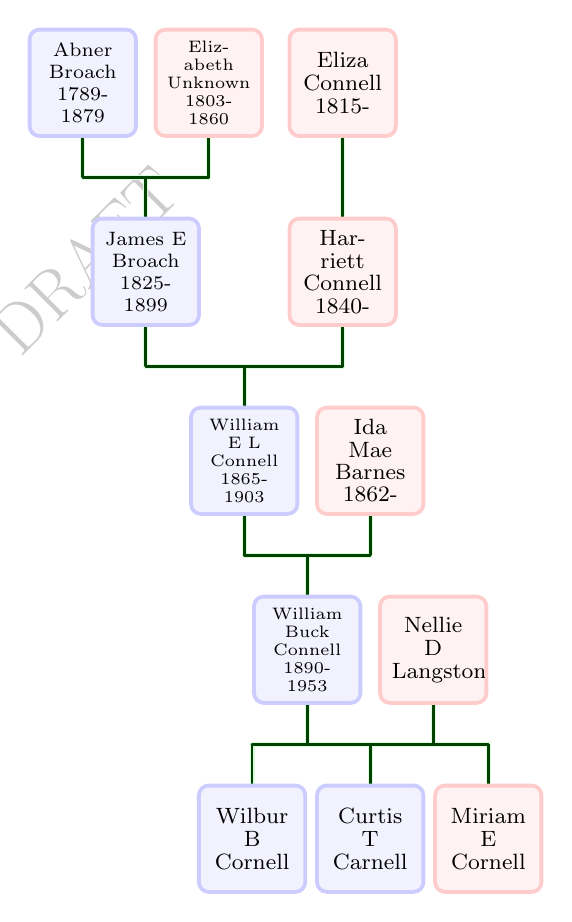
\begin{tikzpicture}
	\genealogytree[
		template=signpost, 
		node size=1.4cm, 
		level size=1.4cm,
		tcbset={male/.style={colframe=blue!20, colback=blue!5},
			female/.style={colframe=red!20, colback=red!5}},
		box={fit basedim=8pt, boxsep=2pt, no shadow}
	]{
		parent{
			c[male]{Wilbur B Cornell}
			g[male]{Curtis T Carnell}
			c[female]{Miriam E Cornell}
			parent{
				g[male]{William Buck Connell\\1890-1953}
				parent{
					g[male]{William E L Connell\\1865-1903}
					parent{
						g[male]{James E Broach\\1825-1899}
						parent{
							g[male]{Abner Broach\\1789-1879}
						}
						parent{
							g[female]{Elizabeth Unknown\\1803-1860}
						}
					}
					parent{
						g[female]{Harriett Connell\\1840-}
						parent{
							g[female]{Eliza Connell\\1815-}
						}
					}
				}
				parent{
					g[female]{Ida Mae Barnes\\1862-}
				}
			}
			parent{
				g[female]{Nellie D Langston}
			}
		}
	}
\end{tikzpicture}

\section{Genealogy}

\input{../tex_output/det_ancestor_report_Connell_mod.tex}

\chapter{Ancestors of Nellie D Langston}

\section{Tree}

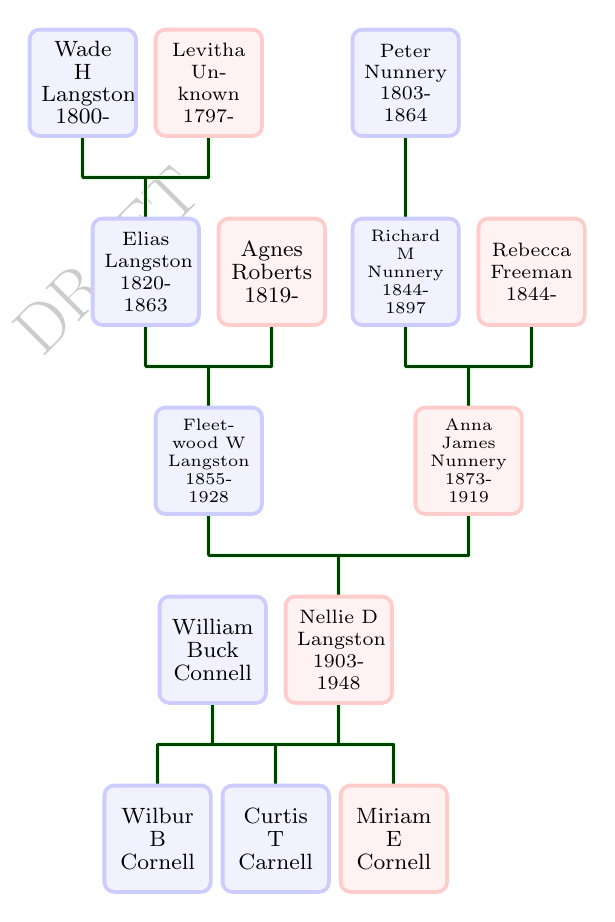
\begin{tikzpicture}
	\genealogytree[
		template=signpost, 
		node size=1.4cm, 
		level size=1.4cm,
		tcbset={male/.style={colframe=blue!20, colback=blue!5},
			female/.style={colframe=red!20, colback=red!5}},
		box={fit basedim=8pt, boxsep=2pt, no shadow}
	]{
		parent{
			c[male]{Wilbur B Cornell}
			g[male]{Curtis T Carnell}
			c[female]{Miriam E Cornell}
			parent{
				g[male]{William Buck Connell}
			}
			parent{
				g[female]{Nellie D Langston\\1903-1948}
				parent{
					g[male]{Fleetwood W Langston\\1855-1928}
					parent{
						g[male]{Elias Langston\\1820-1863}
						parent{
							g[male]{Wade H Langston\\1800-}
						}
						parent{
							g[female]{Levitha Unknown\\1797-}
						}
					}
					parent{
						g[female]{Agnes Roberts\\1819-}
					}
				}
				parent{
					g[female]{Anna James Nunnery\\1873-1919}
					parent{
						g[male]{Richard M Nunnery\\1844-1897}
						parent{
							g[male]{Peter Nunnery\\1803-1864}
						}
					}
					parent{
						g[female]{Rebecca Freeman\\1844-}
					}
				}
			}
		}
	}
\end{tikzpicture}

\section{Genealogy}

\input{../tex_output/det_ancestor_report_Langston_mod.tex}

\chapter{Ancestors of Kendrick Marvin Smith}

\section{Tree}

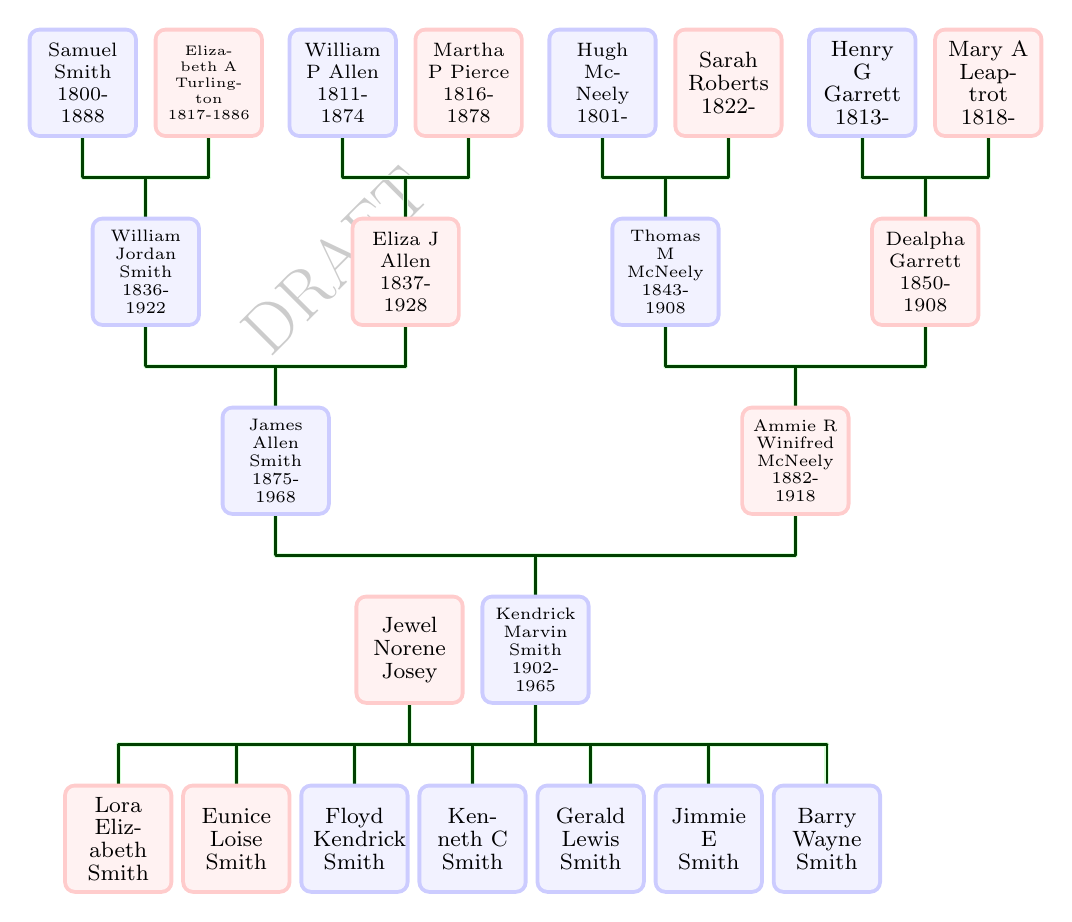
\begin{tikzpicture}
	\genealogytree[
		template=signpost, 
		node size=1.4cm, 
		level size=1.4cm,
		tcbset={male/.style={colframe=blue!20, colback=blue!5},
			female/.style={colframe=red!20, colback=red!5}},
		box={fit basedim=8pt, boxsep=2pt, no shadow}
	]{
		parent{
			g[female]{Lora Elizabeth Smith}
			c[female]{Eunice Loise Smith}
			c[male]{Floyd Kendrick Smith}
			c[male]{Kenneth C Smith}
			c[male]{Gerald Lewis Smith}
			c[male]{Jimmie E Smith}
			c[male]{Barry Wayne Smith}
			parent{
				g[female]{Jewel Norene Josey}
			}
			parent{
				g[male]{Kendrick Marvin Smith\\1902-1965}
				parent{
					g[male]{James Allen Smith\\1875-1968}
					parent{
						g[male]{William Jordan Smith\\1836-1922}
						parent{
							g[male]{Samuel Smith\\1800-1888}
						}
						parent{
							g[female]{Elizabeth A Turlington\\1817-1886}
						}
					}
					parent{
						g[female]{Eliza J Allen\\1837-1928}
						parent{
							g[male]{William P Allen\\1811-1874}
						}
						parent{
							g[female]{Martha P Pierce\\1816-1878}
						}
					}
				}
				parent{
					g[female]{Ammie R Winifred McNeely\\1882-1918}
					parent{
						g[male]{Thomas M McNeely\\1843-1908}
						parent{
							g[male]{Hugh McNeely\\1801-}
						}
						parent{
							g[female]{Sarah Roberts\\1822-}
						}
					}
					parent{
						g[female]{Dealpha Garrett\\1850-1908}
						parent{
							g[male]{Henry G Garrett\\1813-}
						}
						parent{
							g[female]{Mary A Leaptrot\\1818-}
						}
					}
				}
			}
		}
	}
\end{tikzpicture}

\section{Genealogy}

\input{../tex_output/det_ancestor_report_Smith_mod.tex}

\chapter{Ancestors of Jewel Norene Josey}

\section{Tree}

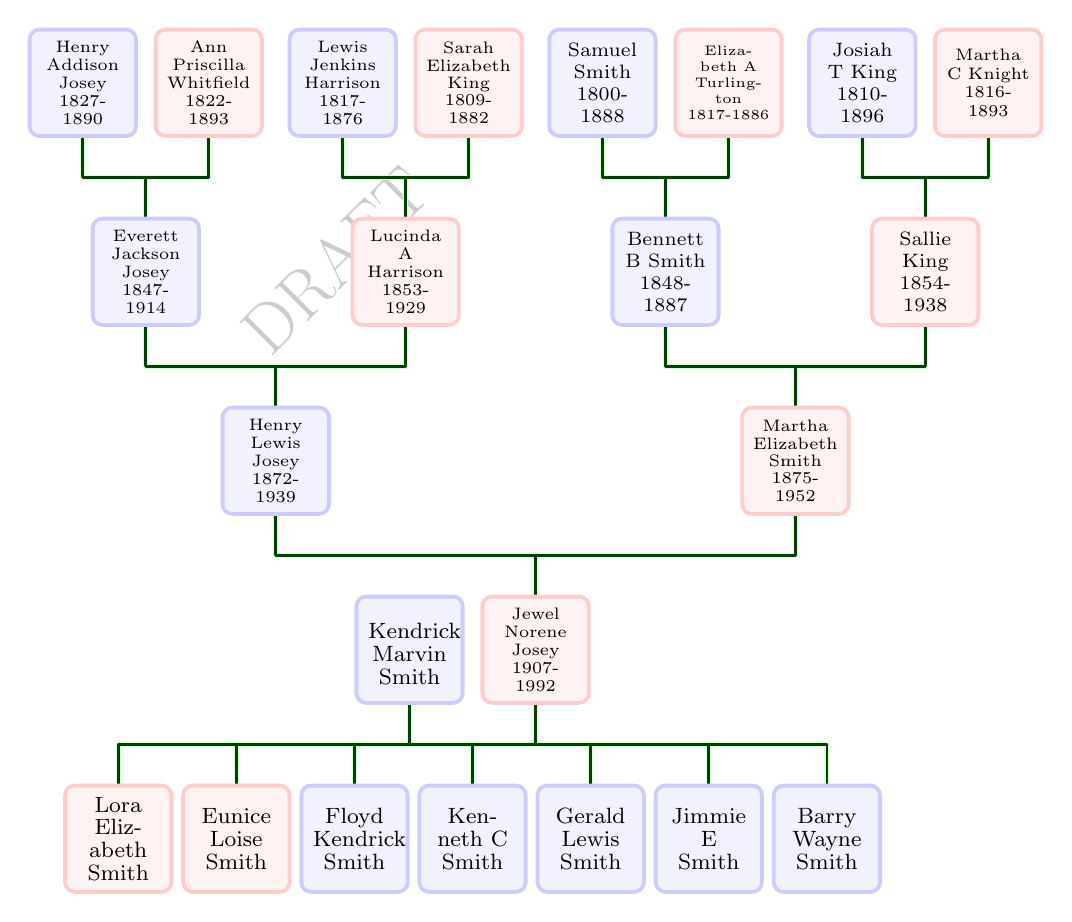
\begin{tikzpicture}
	\genealogytree[
		template=signpost, 
		node size=1.4cm, 
		level size=1.4cm,
		tcbset={male/.style={colframe=blue!20, colback=blue!5},
			female/.style={colframe=red!20, colback=red!5}},
		box={fit basedim=8pt, boxsep=2pt, no shadow}
	]{
		parent{
			g[female]{Lora Elizabeth Smith}
			c[female]{Eunice Loise Smith}
			c[male]{Floyd Kendrick Smith}
			c[male]{Kenneth C Smith}
			c[male]{Gerald Lewis Smith}
			c[male]{Jimmie E Smith}
			c[male]{Barry Wayne Smith}
			parent{
				g[male]{Kendrick Marvin Smith}
			}
			parent{
				g[female]{Jewel Norene Josey\\1907-1992}
				parent{
					g[male]{Henry Lewis Josey\\1872-1939}
					parent{
						g[male]{Everett Jackson Josey\\1847-1914}
						parent{
							g[male]{Henry Addison Josey\\1827-1890}
						}
						parent{
							g[female]{Ann Priscilla Whitfield\\1822-1893}
						}
					}
					parent{
						g[female]{Lucinda A Harrison\\1853-1929}
						parent{
							g[male]{Lewis Jenkins Harrison\\1817-1876}
						}
						parent{
							g[female]{Sarah Elizabeth King\\1809-1882}
						}
					}
				}
				parent{
					g[female]{Martha Elizabeth Smith\\1875-1952}
					parent{
						g[male]{Bennett B Smith\\1848-1887}
						parent{
							g[male]{Samuel Smith\\1800-1888}
						}
						parent{
							g[female]{Elizabeth A Turlington\\1817-1886}
						}
					}
					parent{
						g[female]{Sallie King\\1854-1938}
						parent{
							g[male]{Josiah T King\\1810-1896}
						}
						parent{
							g[female]{Martha C Knight\\1816-1893}
						}
					}
				}

			}
		}
	}
\end{tikzpicture}

\section{Genealogy}

\input{../tex_output/det_ancestor_report_Josey_mod.tex}

\chapter{Endnotes}

\section{Connell Endnotes}

\footnotesize

\input{../tex_output/det_ancestor_report_Connell_mod_notes.tex}

\normalsize

\section{Langston Endnotes}

\footnotesize

\input{../tex_output/det_ancestor_report_Langston_mod_notes.tex}

\normalsize

\section{Smith Endnotes}

\footnotesize

\input{../tex_output/det_ancestor_report_Smith_mod_notes.tex}

\normalsize

\section{Josey Endnotes}

\footnotesize

\input{../tex_output/det_ancestor_report_Josey_mod_notes.tex}

\normalsize

\end{document}
